\section{Current field}

\begin{Exercise}[difficulty=1]
Calculate current density in the wire (circular with diameter 1mm) if total current is 10 A.
\end{Exercise}

\begin{Exercise}[difficulty=2]
Calculate voltage drop on a busbar with rectangular cross-section (1cm by 5cm) made of copper ($57\cdot10^{6}$ S/m. Length of a busbar is 10 meters, and total current if 1000 A.
\end{Exercise}

\begin{Exercise}[difficulty=2]
Find the resistance of wooden pipe filled with water. Assume that conductivity of the water is 1 S/mm, and 0.01 S/m for wood. The pipe is 10 meters long, external radius is 50cm, wall is 5cm thin.
\begin{center}
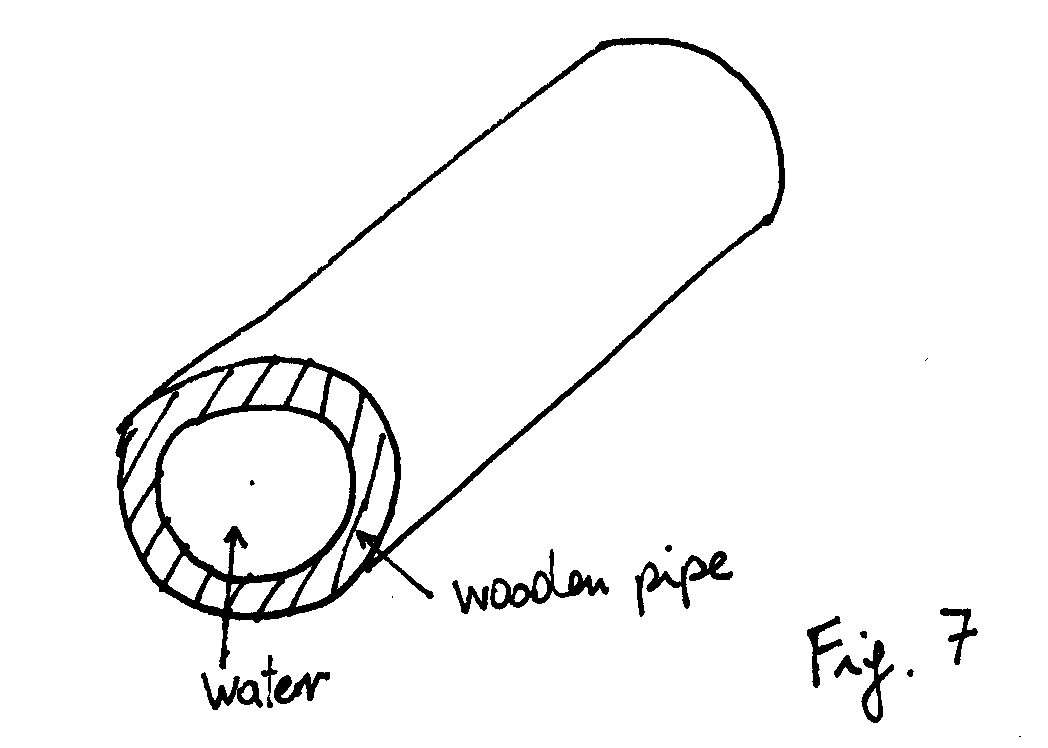
\includegraphics[width=0.4\textwidth]{img/fig_cur1.png} 
\end{center}
\end{Exercise}

\begin{Exercise}[difficulty=3]
Driver is running of the truck which hit high voltage line. Calculate "step potential" if step length is 1m and driver is already 3m from the truck.
\begin{center}
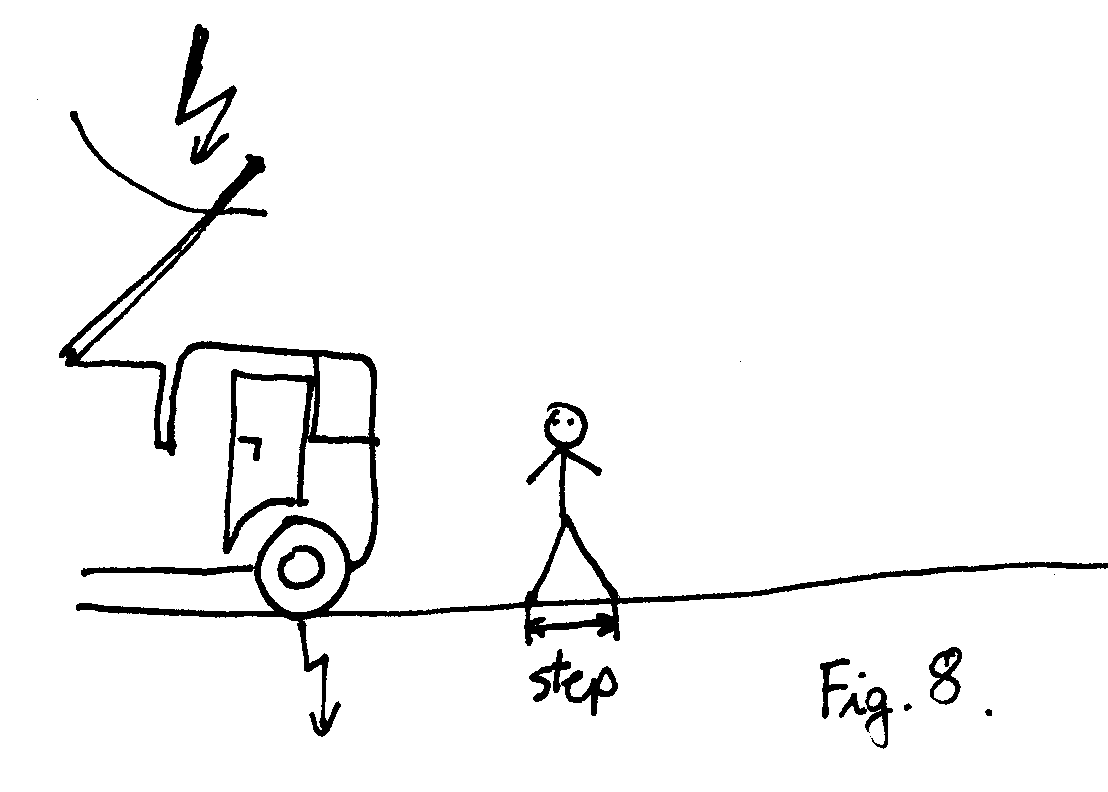
\includegraphics[width=0.4\textwidth]{img/fig_cur2.png} 
\end{center}
\end{Exercise}

\begin{Exercise}[difficulty=2]
Design fuse radius which will blow when the current exceed 20 A. Maximum current density for copper is $10^8$ [A/m].
\end{Exercise}

\begin{Exercise}[difficulty=4]
Calculate resistance between two pipes (radius 0.3 m) floating on the sea surface in the distance 2 meters. Lenght of the pipes is 100 meters. Assume that the conductivity of a sea water is 5 S/m.
\end{Exercise}

